\addcontentsline{toc}{chapter}{Załącznik}
\captionsetup{list=no}
\chapter*{Załącznik}\label{sec:zalacznik}
Ta część pracy została przeznaczona na przybliżenie działania zaimplementowanego systemu i jego interfejsu użytkownika (sekcja \ref{sec:system}). W celu uruchomienia systemu należy pobrać jego kod źródłowy z repozytorium znajdującego się pod adresem: \url{https://github.com/somas3k/casting_dss}. 
W repozytorium znajdują się następujące elementy:
\begin{itemize}
    \item katalog \textit{models} - zawiera pliki modeli wytrenowanych za pomocą algorytmu XGBoost wraz z konfiguracjami warstw wejściowych oraz plik \textit{possible\_values.json} opisujący przestrzeń rozwiązań wygenerowaną dla zbioru danych,
    \item katalog \textit{python\_analysis} - zawiera notebook jupyter o nazwie \textit{optimization\_analyze.ipynb} w którym zapisane są skrypty służące do analizy danych historycznych dla analizy algorytmów,
    \item katalog \textit{src} - zawiera pliki źródłowe programu napisanego w języku Java.
    \item \textit{pom.xml} - plis opisujący zależności projektu oraz sposób budowania wykonywalnego pliku jar.
\end{itemize}

Do zbudowania i uruchomienia projektu potrzebne są następujące elementy:
\begin{itemize}
    \item Java 11 JDK (dostępne pod adresem \url{https://www.openlogic.com/openjdk-downloads}),
    \item Apache Maven (dostępne pod adresem \url{https://maven.apache.org/download.cgi}),
    \item JavaFX 11 SDK (dostępne pod adresem \url{https://gluonhq.com/products/javafx/})
\end{itemize}

Po zaistalowaniu Java 11 i Maven'a należy się upewnić, że oba narzędzia działają. Można to zrobić poprzez wywołanie w wierszu poleceń komend \textit{java --version} i \textit{mvn --version}, które powinny zwrócić zainstalowane wersje. Jeśli wersje są inne należy doprowadzić do sytuacji, by zmienna środowiskowa PATH zawierała poprawne katalogi do plików binarnych JDK i Maven'a. W przypadku Maven'a należy także dodać zmienną środowiskową \textit{JAVA\_HOME}, która będzie wskazywała na katalog z zainstalowanym JDK.

Następnie należy wypakować JavaFX 11 SDK w dowolnym miejscu na dysku i przy pomocy wiersza poleceń przejść do katalogu z pobranym repozytorium. Z poziomu katalogu należy uruchomić polecenie \textit{mvn clean install}, które w rezultacie powinno stworzyć katalog \textit{target} i zakończyć się wiadomością typu: 'BUILD SUCCESS'.

W celu uruchomienia programu należy wywołać następujące polecenie:

\textit{java \-\-module-path \%PATH\_TO\_OPENJFX\_SDK\%/lib \-\-add-modules javafx.controls, javafx.fxml, javafx.graphics -jar ./target/casting\_dss-1.0-SNAPSHOT-jar-with-dependencies.jar}

gdzie wartość \textit{\%PATH\_TO\_OPENJFX\_SDK\%} powinna zostać zastąpiona ścieżką do katalogu z JavaFX 11 SDK, przykład:

\textit{java \-\-module-path /home/kamilw/magisterka/casting\_dss/lib/javafx-sdk-11.0.2/lib \-\-add-modules javafx.controls,javafx.fxml,javafx.graphics -jar ./target/casting\_dss-1.0-SNAPSHOT-jar-with-dependencies.jar}

Poprawne uruchomienie powinno pokazać okno programu z pierwszą otwartą zakładką (rys. \ref{fig:okno1})


\begin{figure}[ht]{}
	\centering
	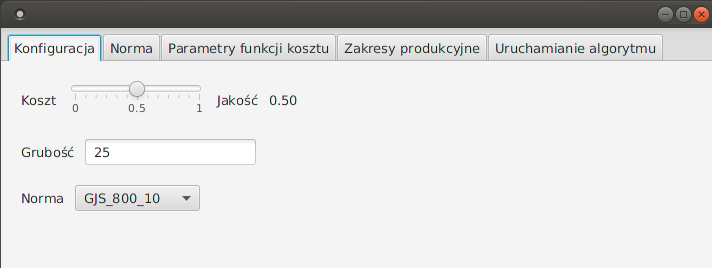
\includegraphics[scale=0.8]{images/okno1.png}
	\caption {
		 Okno aplikacji z otwartą zakładką 'Konfiguracja'.
	}
	\label{fig:okno1}
\end{figure}

Zakładki 'Konfiguracja', 'Norma', 'Parametry funkcji kosztu' oraz 'Zakresy produkcyjne' służą do wprowadzenia danych wejściowych, które zostaną użyte przy optymalizacji.

Najbardziej rozbudowaną częścią systemu jest zakładka 'Uruchamianie algorytmu', której stan początkowy wygląda jak na rys. \ref{fig:initial-state}.

\begin{figure}[ht]{}
	\centering
	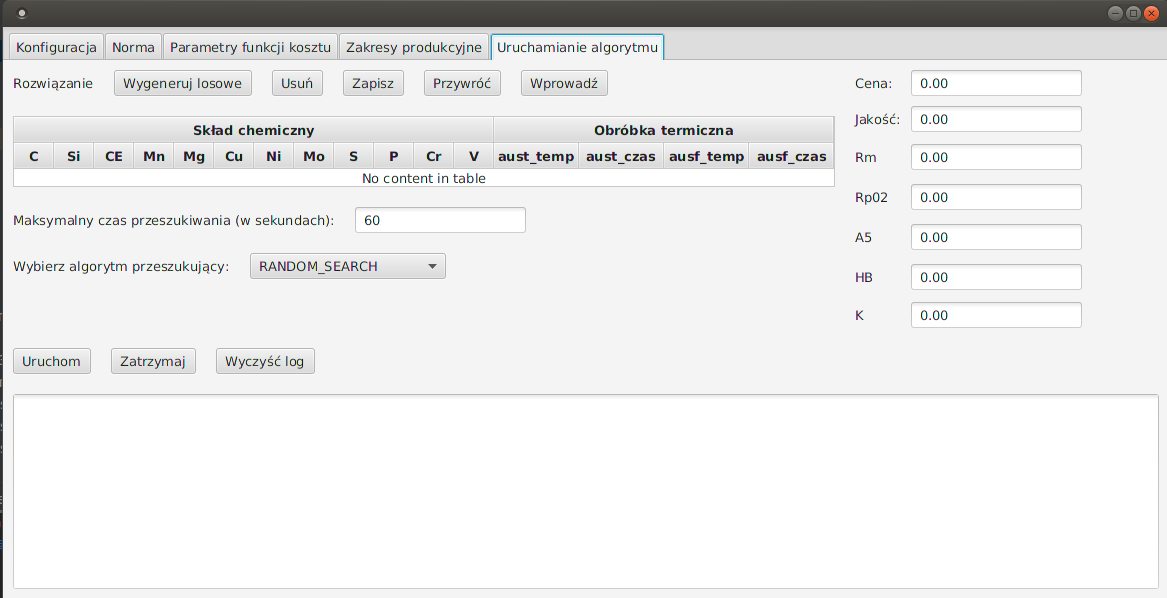
\includegraphics[scale=0.48]{images/initial_state.png}
	\caption {
		 Okno aplikacji z otwartą zakładką 'Uuchamianie algorytmu'.
	}
	\label{fig:initial-state}
\end{figure}

W górnej części okna można zauważyć szereg przycisków. Ich działanie jest następujące:
\begin{itemize}
    \item Wygeneruj losowe - tablica pod rzędem przycisków zostanie wypełniona losowym rozwiązaniem (rys. \ref{fig:random_solution}),
    \item Usuń - usuwa dane z tablicy z rozwiązaniem,
    \item Zapisz - pozwala zachować rozwiązanie tymczasowo w pamięci,
    \item Przywróć - przywraca rozwiązanie, które zostało wcześniej zapisane za pomocą poprzedniego przycisku,
    \item Wprowadź - naciśnięcie tego przycisku skutkuje otwarciem się okna do wprowadzenia swojego rozwiązania (rys. \ref{fig:input}).
    
\end{itemize}

\begin{figure}[ht]{}
	\centering
	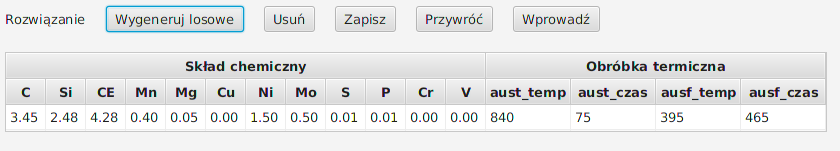
\includegraphics[scale=0.6]{images/random_solution.png}
	\caption {
		 Tablica przedstawiająca aktualne rozwiązanie.
	}
	\label{fig:random_solution}
\end{figure}

\begin{figure}[ht]{}
	\centering
	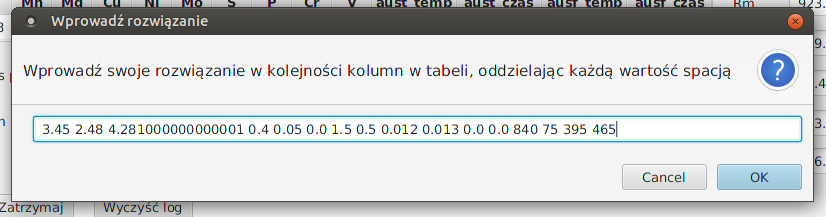
\includegraphics[scale=0.6]{images/input.png}
	\caption {
		 Dialog do wprowadzania rozwiązania.
	}
	\label{fig:input}
\end{figure}

Tablica wyświetlająca aktualny wynik posiada też możliwość wprowadzania zmian po naciśnięciu na wybrane pole.

Dla rozwiązania widniejącego w tablicy są wyświetlane informacje o: Cenie, Jakości, wartości Rm, Rp02, A5, HB i K (rys. \ref{fig:data-view}).

\begin{figure}[ht]{}
	\centering
	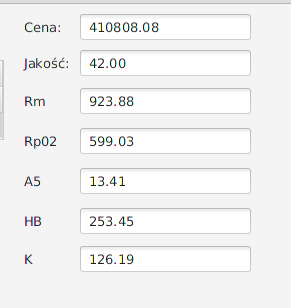
\includegraphics[scale=0.7]{images/data.png}
	\caption {
		 Kontrolki do wyświetlania informacji o koszcie, jakości i wartościach właściwości mechanicznych dla rozwiązania w tabeli.
	}
	\label{fig:data-view}
\end{figure}

W części przedstawionej na rysunku \ref{fig:algo-config} znajdują się kontrolki służące do konfiguracji czasu przeszukiwania, wybrania algorytmu i uruchomienia optymalizacji.

\begin{figure}[ht]{}
	\centering
	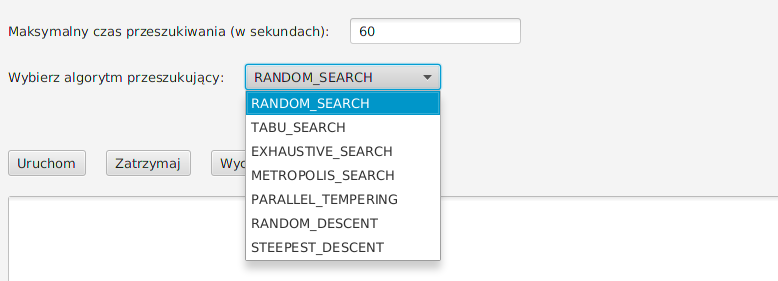
\includegraphics[scale=0.7]{images/algo_config.png}
	\caption {
		 Konfiguracja uruchamiania algorytmu optymalizacji.
	}
	\label{fig:algo-config}
\end{figure}

Po naciśnięciu przycisku 'Uruchom' wybrany algorytm rozpocznie optymalizację i w polu tekstowym u dołu okna zaczną się pojawiać informacje o nowych rozwiązaniach, które będą także wpisywane do tabeli z rozwiązaniem. Przykładowy 'log' został przedstawiony na rys. \ref{fig:algo-log}. Przycisk 'Zatrzymaj' służy do zatrzymania działania algorytmu optymalizacji przed upływem maksymalnego czasu przeszukiwania, a przycisk 'Wyczyść log' służy do wyczyszczenia pola tekstowego z logami.

\begin{figure}[ht]{}
	\centering
	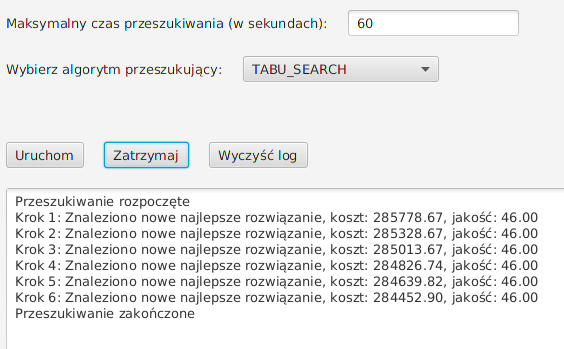
\includegraphics[scale=0.7]{images/algo_log.png}
	\caption {
		 Logi wypisywane podczas procesu optymalizacji.
	}
	\label{fig:algo-log}
\end{figure}